\documentclass[tikz,border=5pt]{standalone}
\usepackage{amsmath,amssymb,bm}
\usetikzlibrary{arrows.meta,calc,positioning}

\definecolor{accent}{RGB}{0, 100, 170}
\definecolor{highlight}{RGB}{200, 60, 30}
\definecolor{darkgreen}{RGB}{0, 120, 60}
\definecolor{earthblue}{RGB}{40,80,150}
\definecolor{orbitgray}{RGB}{100,100,100}

\begin{document}
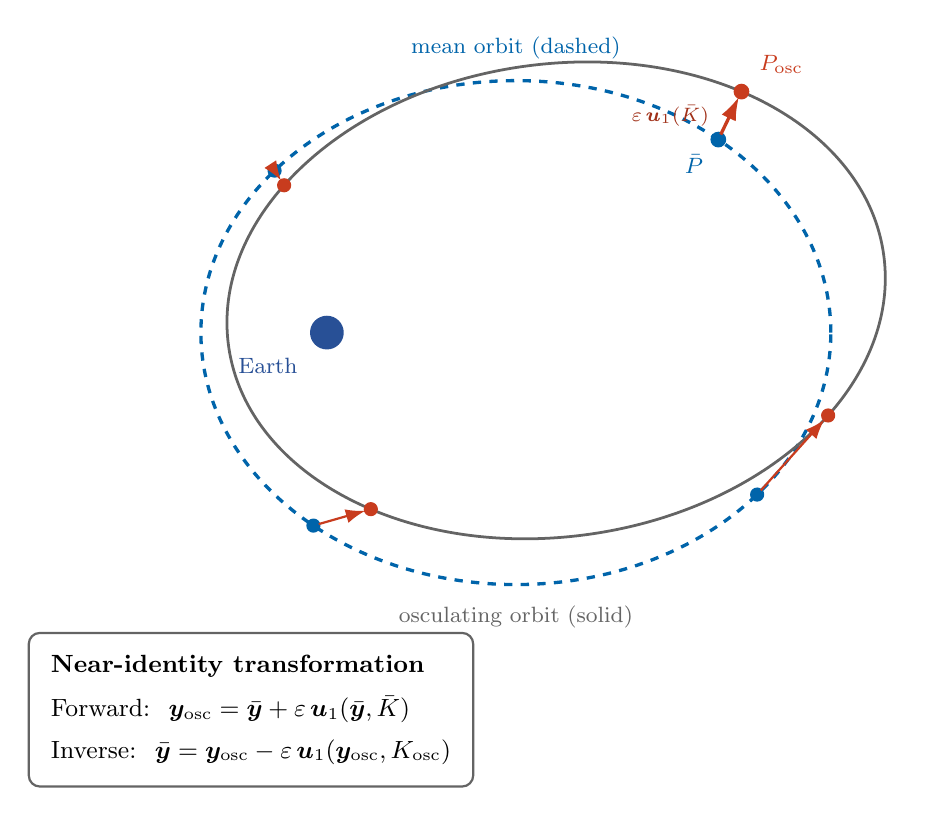
\begin{tikzpicture}[>=Latex, font=\small]

% =====================================================================
% Two ellipses sharing a common focus at the origin.
%
% Mean orbit:      a=4.0, b=3.2 => c=sqrt(16-10.24)=sqrt(5.76)=2.4
%                  center at (2.4, 0), no rotation
% Osculating orbit: a=4.2, b=3.0 => c=sqrt(17.64-9.0)=sqrt(8.64)=2.94
%                  center at (2.94, 0), rotated 8 degrees
%
% Larger difference in eccentricity + more rotation => bigger, more
% visible displacement vectors (the key pedagogical feature).
% =====================================================================

\def\meanA{4.0}
\def\meanB{3.2}
\def\meanCx{2.4}

\def\oscA{4.2}
\def\oscB{3.0}
\def\oscC{2.94}
\def\oscRot{8}

% Mean orbit (dashed accent)
\draw[accent, dashed, thick, line width=1.2pt]
  (\meanCx, 0) ellipse [x radius=\meanA, y radius=\meanB];

% Osculating orbit (solid gray)
\begin{scope}[rotate=\oscRot]
  \draw[orbitgray, thick, line width=1.0pt]
    (\oscC, 0) ellipse [x radius=\oscA, y radius=\oscB];
\end{scope}

% Earth at common focus
\fill[earthblue] (0,0) circle (0.20);
\draw[earthblue, thick] (0,0) circle (0.20);
\node[earthblue, font=\footnotesize, anchor=north east] at (-0.25,-0.2) {Earth};

% Orbit labels — well separated from point clusters
\node[accent, anchor=south, font=\footnotesize] at (2.4, 3.35)
  {mean orbit (dashed)};
\node[orbitgray, anchor=north, font=\footnotesize] at (2.4, -3.35)
  {osculating orbit (solid)};

% =====================================================================
% Displacement vectors at 4 parametric angles.
% Mean point:  (meanCx + meanA*cos(t), meanB*sin(t))
% Osc point:   rotate( (oscC + oscA*cos(t), oscB*sin(t)), oscRot )
% =====================================================================

% --- Position 1: theta=50 (upper right) — primary labelled ---
\pgfmathsetmacro{\tA}{50}
\pgfmathsetmacro{\mxA}{\meanCx + \meanA*cos(\tA)}
\pgfmathsetmacro{\myA}{\meanB*sin(\tA)}
\pgfmathsetmacro{\oxAr}{\oscC + \oscA*cos(\tA)}
\pgfmathsetmacro{\oyAr}{\oscB*sin(\tA)}
\pgfmathsetmacro{\oxA}{\oxAr*cos(\oscRot) - \oyAr*sin(\oscRot)}
\pgfmathsetmacro{\oyA}{\oxAr*sin(\oscRot) + \oyAr*cos(\oscRot)}

\fill[accent] (\mxA, \myA) circle (0.10);
\fill[highlight] (\oxA, \oyA) circle (0.10);
\draw[-{Latex[length=3mm,width=2mm]}, highlight, very thick,
      shorten >=2pt, shorten <=2pt]
  (\mxA, \myA) -- (\oxA, \oyA);
% Labels: P-bar to the left/below, P_osc to the right/above
\node[accent, font=\footnotesize, anchor=north east] at
  ([xshift=-2pt, yshift=-2pt] \mxA, \myA) {$\bar{P}$};
\node[highlight, font=\footnotesize, anchor=south west] at
  ([xshift=3pt, yshift=3pt] \oxA, \oyA) {$P_{\mathrm{osc}}$};
% Displacement label midway, offset away from both labels
\pgfmathsetmacro{\lxA}{0.5*(\mxA + \oxA)}
\pgfmathsetmacro{\lyA}{0.5*(\myA + \oyA)}
\node[highlight!80!black, font=\scriptsize, anchor=east, xshift=-4pt]
  at (\lxA, \lyA) {$\varepsilon\,\bm{u}_1(\bar{K})$};

% --- Position 2: theta=140 (upper left) ---
\pgfmathsetmacro{\tB}{140}
\pgfmathsetmacro{\mxB}{\meanCx + \meanA*cos(\tB)}
\pgfmathsetmacro{\myB}{\meanB*sin(\tB)}
\pgfmathsetmacro{\oxBr}{\oscC + \oscA*cos(\tB)}
\pgfmathsetmacro{\oyBr}{\oscB*sin(\tB)}
\pgfmathsetmacro{\oxB}{\oxBr*cos(\oscRot) - \oyBr*sin(\oscRot)}
\pgfmathsetmacro{\oyB}{\oxBr*sin(\oscRot) + \oyBr*cos(\oscRot)}

\fill[accent] (\mxB, \myB) circle (0.09);
\fill[highlight] (\oxB, \oyB) circle (0.09);
\draw[-{Latex[length=2.5mm,width=1.8mm]}, highlight, thick,
      shorten >=2pt, shorten <=2pt]
  (\mxB, \myB) -- (\oxB, \oyB);

% --- Position 3: theta=230 (lower left) ---
\pgfmathsetmacro{\tC}{230}
\pgfmathsetmacro{\mxC}{\meanCx + \meanA*cos(\tC)}
\pgfmathsetmacro{\myC}{\meanB*sin(\tC)}
\pgfmathsetmacro{\oxCr}{\oscC + \oscA*cos(\tC)}
\pgfmathsetmacro{\oyCr}{\oscB*sin(\tC)}
\pgfmathsetmacro{\oxC}{\oxCr*cos(\oscRot) - \oyCr*sin(\oscRot)}
\pgfmathsetmacro{\oyC}{\oxCr*sin(\oscRot) + \oyCr*cos(\oscRot)}

\fill[accent] (\mxC, \myC) circle (0.09);
\fill[highlight] (\oxC, \oyC) circle (0.09);
\draw[-{Latex[length=2.5mm,width=1.8mm]}, highlight, thick,
      shorten >=2pt, shorten <=2pt]
  (\mxC, \myC) -- (\oxC, \oyC);

% --- Position 4: theta=320 (lower right) ---
\pgfmathsetmacro{\tD}{320}
\pgfmathsetmacro{\mxD}{\meanCx + \meanA*cos(\tD)}
\pgfmathsetmacro{\myD}{\meanB*sin(\tD)}
\pgfmathsetmacro{\oxDr}{\oscC + \oscA*cos(\tD)}
\pgfmathsetmacro{\oyDr}{\oscB*sin(\tD)}
\pgfmathsetmacro{\oxD}{\oxDr*cos(\oscRot) - \oyDr*sin(\oscRot)}
\pgfmathsetmacro{\oyD}{\oxDr*sin(\oscRot) + \oyDr*cos(\oscRot)}

\fill[accent] (\mxD, \myD) circle (0.09);
\fill[highlight] (\oxD, \oyD) circle (0.09);
\draw[-{Latex[length=2.5mm,width=1.8mm]}, highlight, thick,
      shorten >=2pt, shorten <=2pt]
  (\mxD, \myD) -- (\oxD, \oyD);

% ===== EQUATION BOX (bottom left, clear of the orbits) =====
\node[draw=orbitgray, rounded corners=4pt, fill=white,
      inner sep=8pt, anchor=north west, font=\small, align=left,
      line width=0.8pt]
  at (-3.8, -3.8) {%
  \textbf{Near-identity transformation}\\[5pt]
  Forward:\; $\bm{y}_{\mathrm{osc}} = \bar{\bm{y}}
    + \varepsilon\,\bm{u}_1(\bar{\bm{y}}, \bar{K})$\\[4pt]
  Inverse:\; $\bar{\bm{y}} = \bm{y}_{\mathrm{osc}}
    - \varepsilon\,\bm{u}_1(\bm{y}_{\mathrm{osc}}, K_{\mathrm{osc}})$};

\end{tikzpicture}
\end{document}
